\section{Struktogramm}

Nassi–Shneiderman Diagramme/Struktgramme werden verwendet, um eine Funktion eines Programmes zu visualisieren. 
Dafür gibt es verschiedene Grafische Elemente, welche man dann direkt in Quellcode übertragen kann.

Ein Beispiel:

\vspace{2mm}

\begin{center}
    \ifthenelse{\boolean{svgWorks}}{
        \includesvg[width = \linewidth, inkscapelatex=false]{svg/Struktogramm_bsp.svg}    
    }{
        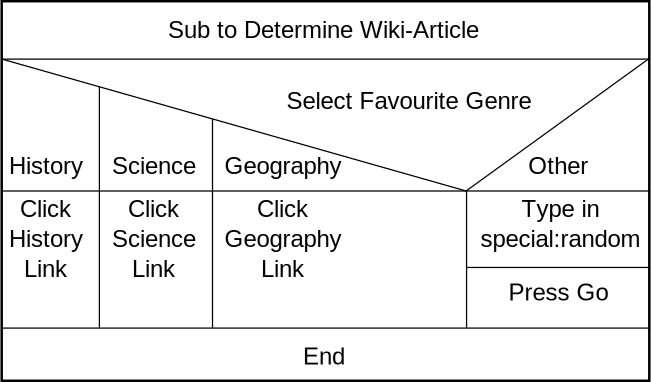
\includegraphics[width=1\columnwidth]{Pictures/Struktogramm_bsp.png}
        }
\end{center}

\subsection{Sinnbilder in C}

Es gibt verschiedene Sinnbilder für verschiedene Funktionen in C. 
Sie können auch ineinander verschachtelt werden:

\subsubsection{Prozessblöcke}

Eine Anweisung, die nach einem Block abgearbeitet wird, ist in einem Rechteck unter dem Block.

\vspace{2mm}
\noindent
\begin{minipage}[c]{0.45\columnwidth}
    \begin{center}
        \ifthenelse{\boolean{svgWorks}}{
            \includesvg[width = 0.5\linewidth, inkscapelatex=false]{svg/Struktogramm_Prozessbloecke.svg}    
        }{
            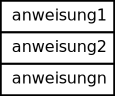
\includegraphics[width=1\columnwidth]{Pictures/Struktogramm_Prozessbloecke.png}
            }
    \end{center}
\end{minipage}
\begin{minipage}[c]{0.45\columnwidth} 
\begin{lstlisting}[language = c]
    anweisung1;
    anweisung2;
    anweisungn;
\end{lstlisting}
\end{minipage}

\subsubsection{Decision / if}

Eine Decision wird wie folgt realisiert.
Wenn kein else verwendet wird kann der Block leer sein.

\vspace{2mm}
\noindent
\begin{minipage}[c]{0.6\columnwidth} 
    \begin{center}
        \ifthenelse{\boolean{svgWorks}}{
            \includesvg[width = \linewidth, inkscapelatex=false]{svg/Struktogramm_decision.svg}    
        }{
            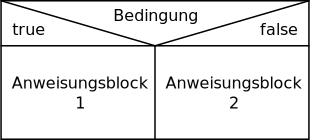
\includegraphics[width=1\columnwidth]{Pictures/Struktogramm_decision.png}
            }
    \end{center}
\end{minipage}
\begin{minipage}[c]{0.4\columnwidth} 
\begin{lstlisting}[language = c]
if(bedingung)
{
    Anweisungsblock 1;
}
else
{
    Anweisungsblock 2;
}
\end{lstlisting}
\end{minipage}

\subsubsection{switch}

\noindent
\begin{minipage}{0.6\columnwidth}
    \begin{center}
        \ifthenelse{\boolean{svgWorks}}{
            \includesvg[width = \linewidth, inkscapelatex=false]{svg/Struktogramm_switch.svg}    
        }{
            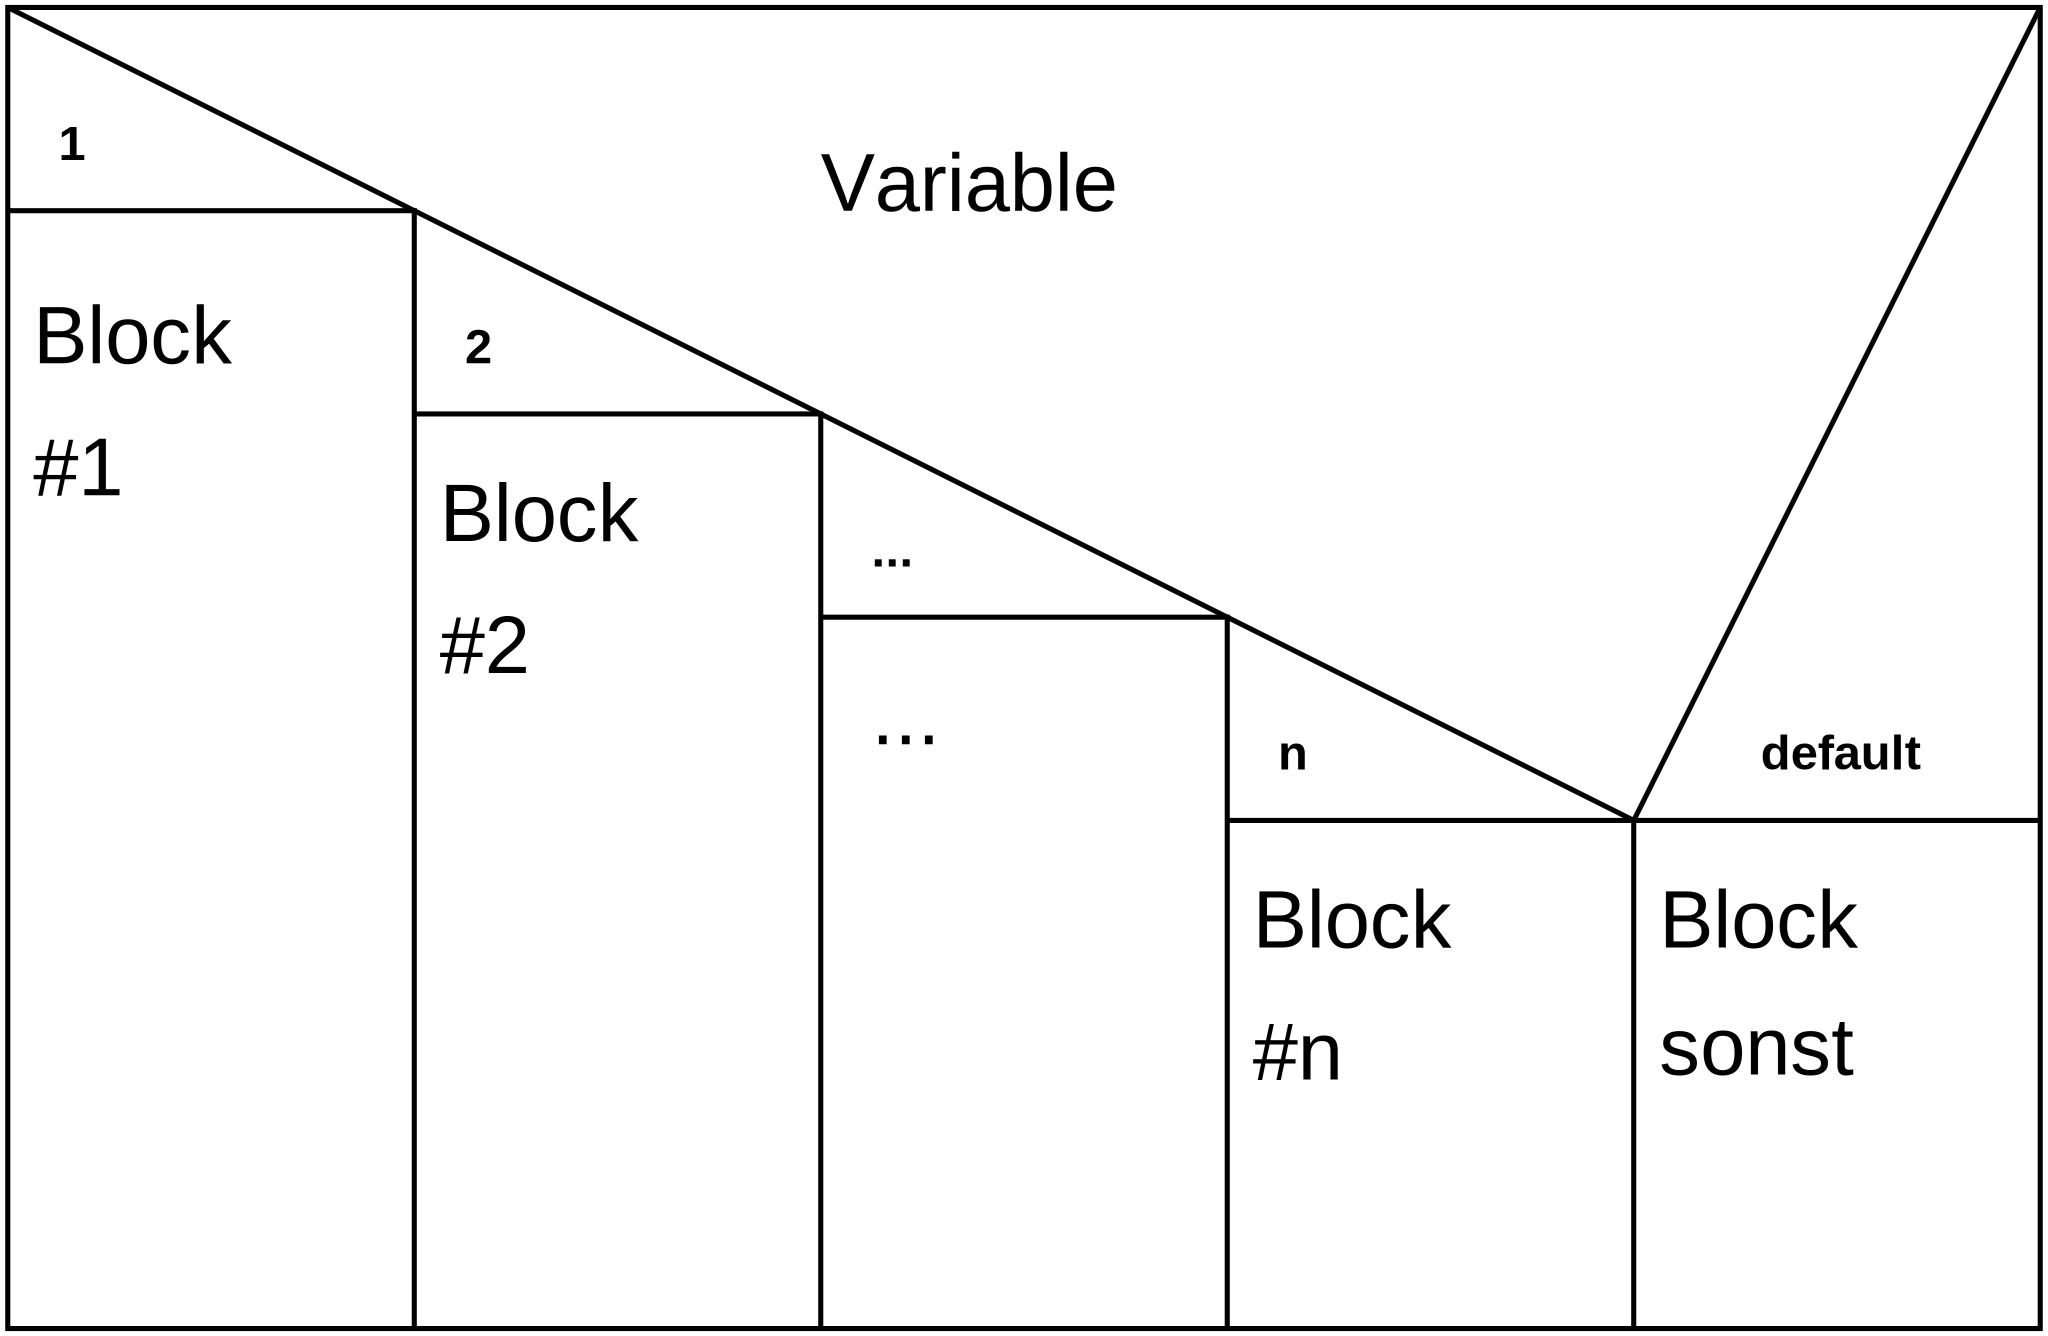
\includegraphics[width=1\columnwidth]{Pictures/Struktogramm_switch.png}
            }
    \end{center}
\end{minipage}
\begin{minipage}{0.3\columnwidth} 
\begin{lstlisting}[language = c]
switch(variable)
{
    case 1:
        block1;
        break;
    case 2:
        block2;
        break;
    case n:
        blockn;
        break;
    default:
        blocksonst;
        break;
}
\end{lstlisting}
\end{minipage}

\subsubsection{for}

\noindent
\begin{minipage}{0.6\columnwidth}
    \begin{center}
        \ifthenelse{\boolean{svgWorks}}{
            \includesvg[width = \linewidth, inkscapelatex=false]{svg/Struktogramm_for.svg}    
        }{
            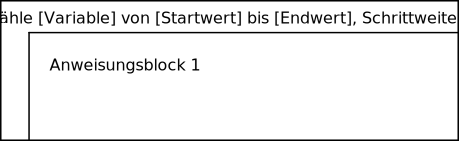
\includegraphics[width=1\columnwidth]{Pictures/Struktogramm_for.png}
            }
    \end{center}
\end{minipage}
\begin{minipage}{0.4\columnwidth} 
\begin{lstlisting}[language = c]
for(int i = Startwert;i< Endwert;i+=1)
{
    anweisungsblock1;
}
\end{lstlisting}
\end{minipage}

\subsubsection{while}

\noindent
\begin{minipage}{0.4\columnwidth}
    \begin{center}
        \ifthenelse{\boolean{svgWorks}}{
            \includesvg[width = \linewidth, inkscapelatex=false]{svg/Struktogramm_while.svg}    
        }{
            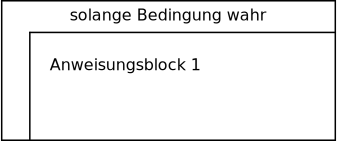
\includegraphics[width=1\columnwidth]{Pictures/Struktogramm_while.png}
            }
    \end{center}
\end{minipage}
\begin{minipage}{0.6\columnwidth} 
\begin{lstlisting}[language = c]
while(bedingung)
{
    anweisungsblock1;
}
\end{lstlisting}
\end{minipage}

\subsubsection{do while}

\noindent
\begin{minipage}{0.4\columnwidth}
    \begin{center}
        \ifthenelse{\boolean{svgWorks}}{
            \includesvg[width = \linewidth, inkscapelatex=false]{svg/Struktogramm_doWhile.svg}    
        }{
            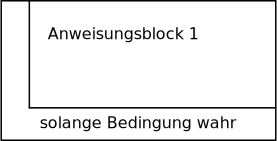
\includegraphics[width=1\columnwidth]{Pictures/Struktogramm_doWhile.png}
            }
    \end{center}
\end{minipage}
\begin{minipage}{0.6\columnwidth} 
\begin{lstlisting}[language = c]
do
{
    anweisungsblock1;
}
while(bedingung);
\end{lstlisting}
\end{minipage}

\nextcol		
